
\begin{marginfigure}
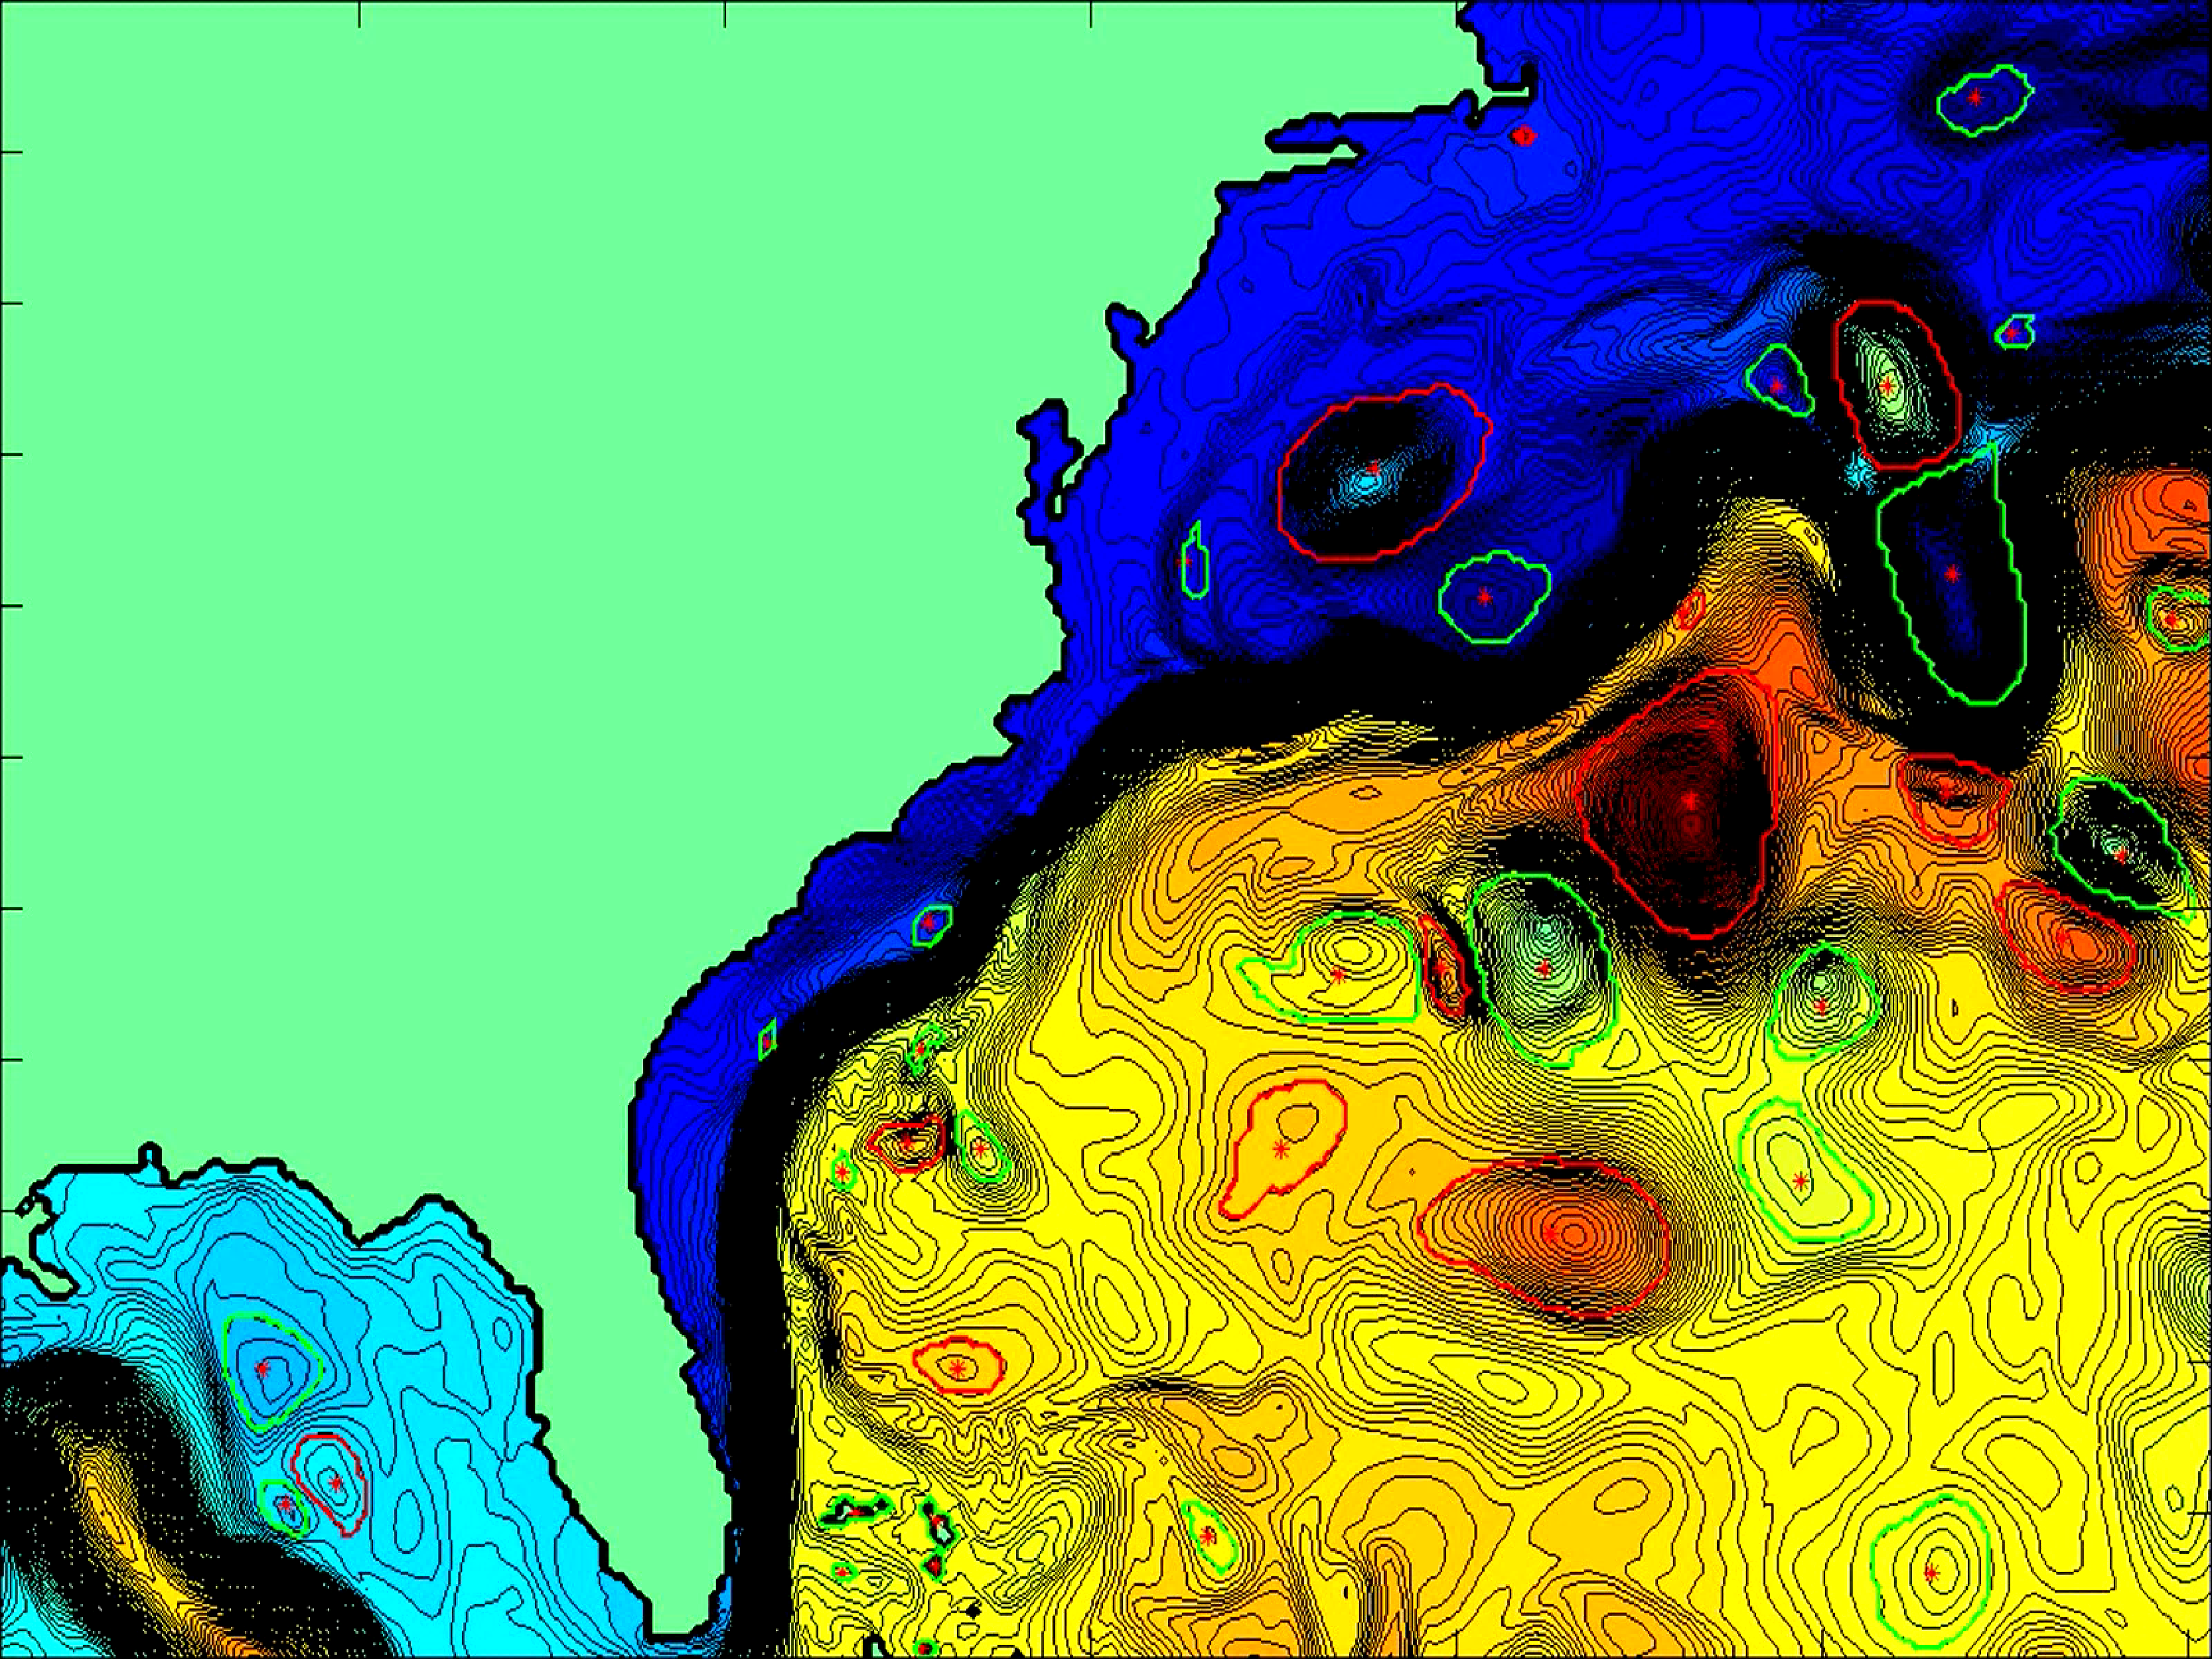
\includegraphics[]{GS.pdf}
\caption{Animation snapshot of early test run. Shown is \SSH~with detected eddies indicated by red and green lines.}
\end{marginfigure}

%\newthought{This } section discusses the theory of meso-scale turbulence and parametrizations thereof.
\newthought{Geostrophic } turbulence is typically characterized by rather stable, often deep reaching, more or less circular, coherent pressure anomalies that rotate fluid around in a vortex in quasi-geostrophic equilibrium \citep{Zhang2013}. These entities can persist for long periods of time in which they often travel distances on the order of hundreds of kilometers
zonally. The fact that baroclinic instability leads to these vortices, instead of cascading to ever smaller scales as would be expected from chaotic
turbulence, is a direct consequence of the inverse energy cascade of two-dimensional motion \footnote{For a discussion of this phenomenon see~\cref{chap:turbu_categories}} (see~\cref{fig:PSI}.) \citep{Rhines1979,Meneguzzis1988}.
The atmospheric analog are storms and high-pressure systems, yet with much less difference between high- and low-pressure systems due to
a smaller centrifugal force \ie smaller Rossby number ($\Ro$). These quasi-geostrophic, mesoscale vortices, from here on called eddies \footnote{For a discussion of
the different types of vortices in the ocean see appendix \cref{chap:eddy_cat}}, are immediately visible on SSH-maps (see~\cref{fig:SSHB}). Yet, it is difficult to physically \emph{define} an eddy in terms of oceanographic variables. The transition from meandering jets or other undeveloped
baroclinic turbulence to a coherent vortex is not very sharp. Eddies also sometimes merge or split or collectively form rifts and valleys in SSH. Detecting them on one snapshot automatically via an algorithm is therefore not trivial. Further problems arise when the algorithm is also supposed to track each individual eddy over time. Their sheer abundance at any
given time inevitably creates ambiguities  as to \textit{which is which} between time steps. 


\subsection{Detection Methods} \label{subsec:detectmethods}
\begin{itemize}

	\item
	One way to find an eddy in SSH-data is to simply scan for closed contours at different values for $\vec{z}$ and then subject found entities to a series of geometric tests to decide whether the contour qualifies. Only if all criteria are met is an eddy found. This method was first used by \citet{Chelton2011} and is certainly a relatively simple yet very effective method, at least so for satellite data. Therefore, as a starting point, this method will be adopted and should also serve as a general definition of what will be referred to as an \textit{eddy} hereafter.
	
\newthought{\citeauthor{Chelton2011} } set the following threshold criteria for their algorithm:
	\begin{enumerate}
		\item
		The \SSH~values of all of the pixels are above (below) a given \SSH~threshold for anticyclonic (cyclonic) eddies.
		\item
		There are at least \textit{[threshold]} pixels and fewer than \textit{[threshold]} pixels comprising the connected region.
		\item
		There is at least one local maximum (minimum) of \SSH~for anticyclonic (cyclonic) eddies.
		\item
		The amplitude of the eddy is at least \textit{[threshold]}.
		\item
		The distance between any pair of points within the connected region must be less than \textit{[threshold]}.
	\end{enumerate}

\item
Another frequently used method to define an eddy makes use of the 2d deformation tensor $\grad \vec{u}$.
\begin{align}
det(\lambda\vec{I}- \vec{\grad \vec{u}}) =0 \label{eq:OWa}
\end{align}
The Sign of its squared eigenvalues indicates whether the flow-field has parabolic, vorticity dominated character, or whether deformation dominates, giving hyperbolic character. Expanding \eqref{eq:OWa} yields
\begin{align}
%\left( \lambda - u_{x} \right) \left( \lambda - v_{y} \right) - u_{y} v_{x}
%&=
%0 \nonumber\\
%%
%\lambda^{2} -\lambda v_{y} -\lambda u_{x} + u_{x} v_{y} - u_{y} v_{x}
%&=
%0 \nonumber \\
%%%
\lambda^{2}
-\lambda
\left( v_{y} + u_{x} \right)
+ u_{x} v_{y}
- u_{y} v_{x}
&=
0 \label{eq:OWb}
\end{align}
Assuming horizontal velocities to be much larger than vertical \ie applying the small aspect-ratio assumption \citep{olbers2012ocean}, the motion becomes 2-dimensional and the continuity equation reduces to $u_{x} = -v_{y}$. Hence 
\begin{align}
%\lambda^{2}
%+ u_{x} v_{y}
%- u_{y} v_{x}
%&=
%0 \nonumber \\
%\lambda^{2}
%- u_{x}^{2}
%- u_{y} v_{x}
%&=
%0 \nonumber \\
\lambda^{2}
&=
\okubo/4
=
 u_{x}^{2}
 +u_{y} v_{x} \label{eq:OWc}
\end{align}
	This is called the Okubo-Weiss-Parameter \footnote{see also \cref{der:okubo}} $\okubo$ \citep{Okubo1970}.
Its meaning is further elucidated by interpreting \eqref{eq:OWc} as
\begin{align}
\okubo	
	&=
	s_{n}^{2}
	+
	s_{s}^{2}
	-
	\omega^{2} \\
	&=
	\left( u_{x} - v_{y} \right)^{2}
	+
	\left( v_{x} + u_{y} \right)^{2}
	-
	\left( v_{x} - u_{y} \right)^{2} \nonumber \\
	&=
	\left( u_{x}^{2} - 2u_{x}v_{y} + v_{y}^{2}\right)
	+
	\left( v_{x}^{2} + 2v_{x}u_{y} + u_{y}^{2}\right)
	-
	\left( v_{x}^{2} - 2v_{x}u_{y} + u_{y}^{2}\right) \nonumber \\
	&=
	\left( u_{x}^{2} - 2u_{x}v_{y} + v_{y}^{2}\right)
	+
 4v_{x}u_{y}\nonumber \\
	&=
	\left( u_{x}^{2} + 2u_{x}^{2} + u_{x}^{2}\right)
	+
 4v_{x}u_{y}\nonumber \\
	&=
4 u_{x}^{2} 
	+
 4v_{x}u_{y} \nonumber
\end{align}
where $s_{n/s}$ are the normal respective shear components of strain. Its sign thus describes the field's tendency for either vorticity- or shear-dominated motion \citep{Isern-Fontanet2006}.
	 An area of large negative values of $\okubo$ indicates high enstrophy density compared to gradients of kinetic energy \cite{Weiss1991}, thus indicating little friction paired with high momentum \ie a vorticity dominated field as would be found in a coherent, angular-momentum-conserving entity. Positive values on the other hand indicate motion dominated by deformation as \eg in-between two vortices of opposite sign.
	 
	 \newthought{As } useful as this parameter seems, it turns out that using it to identify eddies is often not practical.
	\Citet{Chelton2011} name 3 major drawbacks:
	\begin{itemize}
		\item
		\textit{ No single threshold value for $\okubo$ is optimal for the entire World Ocean. Setting the threshold too high can result in failure to identify small eddies, while a threshold that is too low can lead to a definition of eddies with unrealistically large areas that may encompass multiple vortices, sometimes with opposite polarities. }
		\item
		$\okubo$ is highly susceptible to noise in the \SSH~field. Especially when velocities are calculated from geostrophy, the sea surface has effectively
		been differentiated twice and then squared, exacerbating small incontinuities in the data.
		\item
		\textit{The third problem with the W-based method is that the interiors of eddies defined by closed contours of W do not generally coincide with closed contours of SSH. The misregistration of the two fields is often quite substantial. }
	\end{itemize}
	In summary, the $\okubo$-method critically hinges on the necessary assumption of a smooth, purely geostrophic \SSH~topography and is therefor inferior to the approach of scanning for closed SSH-contours directly (as was done so by \citeauthor{Chelton2011}) (see also \citet{Zhang2013}).



\end{itemize}
\newpage
